\documentclass[12pt]{article}

\usepackage{fancyhdr}
\usepackage{amsthm}
\usepackage{amsmath}
\usepackage{graphicx}
\usepackage{amssymb}
\usepackage{esint}
\usepackage{subfigure}
\usepackage{color}
\usepackage{moreverb}
\usepackage{wrapfig}

\textwidth 17cm \topmargin -1cm \oddsidemargin 0cm \textheight 21.5cm
\pagestyle{empty} \pagestyle{fancyplain}
\lhead[\fancyplain{}{}]{\fancyplain{}{{\sc Adam Farnsworth, Myles Adams:}}}
\chead[\fancyplain{}{}]{\fancyplain{}{{\sc Hw 3}}}
\rhead[\fancyplain{}{}]{\fancyplain{}{{\sc Fall 2017}}}

\newcommand{\etal}{\textit{et al. }}

\begin{document}
\centerline{\Large\textbf{Homework 3}}
\vspace{2cm}

\section*{Introduction}\label{sec::Intro}
The goal of this project is to simulate the flow around a rotating cylinder.  The two spatial directions domain is $\Omega = (x_L, x_R) X(t_B,Y_T)$ with a time interval of $[t_{start}, t_{final}]$, velocity vector $\overrightarrow{v} = \begin{bmatrix}
           v_x \\
          v_y \\
         \end{bmatrix}$ and a function $c = c(t,x,y)$ satisfying the advection equation below:\\
\begin{center}
$
\frac{\partial c}{\partial t} + \overrightarrow{v} \cdot \bigtriangledown c = f(t,x,y)$, for all $(x,y)$ $ \in$ $ \Omega$ and $ t$ $ \in$ $ [t_{start},t_{final}]$
\end{center}
with boundary conditions:\\
\begin{center}
$c(t,x,y) = g(t,x,y)$, for all $(x,y)$ $ \in$ $ \Omega$ and $ t$ $ \in$ $ [t_{start},t_{final}]$
\end{center}
where $\partial \Omega$ is the boundary of domain $\Omega$, and initial data:
\begin{center}
$c(t_{start},x,y) = c_{start}(x,y)$, for all $(x,y)$ $ \in$ $ \Omega$
\end{center}
where $f(t,x,y), g(t,x,y)$ and $c_{start}(x,y)$ are given functions.



\section{Problem 1}\label{sec::Problem 1}

\subsection{Part a}\label{sec::a}
Implementing the upwind scheme for this problem with the following example:

\begin{eqnarray}
\textrm{Domain:}\quad \quad \quad \quad \quad \quad \quad \quad \quad \Omega &=& [-1;1]X[-1;1]  \\\nonumber
\textrm{Velocity field: }\quad \quad \quad v_x(t,x,y) &=& -y\\\nonumber
			 v_y(t,x,y) &=& x\\\nonumber
\textrm{Source term:}\quad \quad \quad \quad f(t,x,y)&=&0 \\\nonumber
\textrm{Boundary conditions: } g(t,x,y)&=&0 \\\nonumber
\textrm{Initial conditions: }\quad c_{start}(x,y)&=&\frac{1}{2}\left(1-\tanh \left( \frac{\sqrt{(x-R)^2+y^2}-r}{\epsilon}\right)\right)\\\nonumber 
\end{eqnarray}
where $r=0.2$, $R=0.5$, and $\epsilon = 0.1$. The exact solution in this case is given by:
\begin{center}
$ c_{exact}(t,x,y)=\frac{1}{2}\left(1-\tanh \left( \frac{\sqrt{(x-R \cos(t))^2+(y\sin(t))^2}-r}{\epsilon}\right)\right)$
\end{center}
The advection equation from $t_{start}=0$ to $t_{final} = 0.2$ using grid resolutions $N_x = N_y = 50, 100, 200, 400$ and the Courant number $C=0.75$ is solved by discretizing the interval $[x_L, x_R]$ into a grid of $N_x$ points:
\begin{center}
$ x_1 = x_L, \quad x_2 = x_1 + \Delta x, \quad x_3 = x_2 + \Delta x, \quad ..., \quad x_{N_x}=x_R$
\end{center}
with spatial step
\begin{center}
$ \Delta x = \frac{x_R-x_L}{N_x-1}$
\end{center}
and also discretizing the interval $[y_B, y_T]$ into a grid of $N_y$ points:
\begin{center}
$ y_1 = y_B, \quad y_2 = y_1 + \Delta y, \quad y_3 = y_2 + \Delta y, \quad ..., \quad y_{N_y}=y_T$
\end{center}
with spatial step
\begin{center}
$ \Delta y = \frac{y_T-y_B}{N_y-1}$
\end{center}
The approximate $c(t,x,y)$ as a set of $N_x$ and $N_y$ values where $c_{i,j}(t), i = 1, ..., N_x , j =1,...,N_j$ denotes approximate values of function $c(t,x,y)$ at grid points $x_i, i =1,...,N_x$ and $x_j = 1,...,N_y$.  The values of function $c(t,x,y)$ at time $t =  t_{start}$ at all grid points is given by the initial conditions:
\begin{center}
$ c_1(t_{start}) = c_{start}(x_1,y_1), \quad c_2(t_{start}) = c_{start}(x_2,y_2), \quad ..., \quad c_{N_x}(t_{start}) = c_{start}(x_1{N_x},y_{N_y})$
\end{center}
The spatial derivative $\frac{\partial c}{\partial x} (t,x_i, y_j)$ and $\frac{\partial c}{\partial y} (t,x_i, y_j)$ at grid point $x_i, y_j$ can be approximated using values of function $c(t,x,y)$ at the same point $x_i, y_j$ and its neighboring points.  Forward difference and backward difference will be used for this task:
\begin{eqnarray}
\textrm{Forward difference: } \frac{\partial c}{\partial x}(t,x_i,y_j) &=& \frac{c(t,x_{i+1},y_j-c(t,x_i,y_j)}{\Delta x} + O(\Delta x) \\\nonumber
\frac{\partial c}{\partial y}(t,x_i,y_j)&=&\frac{c(t,x_{i},y_{j+1}-c(t,x_i,y_j)}{\Delta y} + O(\Delta y) \\\nonumber
\textrm{Backward difference: } \frac{\partial c}{\partial x}(t,x_i,y_j) &=& \frac{c(t,x_{i},y_j-c(t,x_{i-1},y_j)}{\Delta x} + O(\Delta x) \\\nonumber
\frac{\partial c}{\partial y}(t,x_i,y_j)&=&\frac{c(t,x_{i},y_{j}-c(t,x_i,y_{j-1})}{\Delta y} + O(\Delta y) \\\nonumber
\end{eqnarray}
From these we can get an approximation called the upwind discretization below:
\begin{center}
$v_x\frac{\partial c}{\partial x}(t,x_i,y_j)\approx\begin{cases} 
v\frac{c(t,x_i,y_j)-c(t,x_{i-1},y_j)}{\Delta x}, \textrm{if }v(t,x_i,y_j) \geq 0 \\
v\frac{c(t,x_{i+1},y_j)-c(t,x_{i},y_j)}{\Delta x}, \textrm{if }v(t,x_i,y_j) < 0 \\
 \end{cases}
$
\end{center}
\begin{center}
$v_y\frac{\partial c}{\partial y}(t,x_i,y_j)\approx\begin{cases} 
v\frac{c(t,x_i,y_j)-c(t,x_{i},y_{j-1})}{\Delta t}, \textrm{if }v(t,x_i,y_j) \geq 0 \\
v\frac{c(t,x_{i},y_{j+1})-c(t,x_{i},y_j)}{\Delta y}, \textrm{if }v(t,x_i,y_j) < 0 \\
 \end{cases}
$
\end{center}
The CFL stability condition for the 2D upwind scheme is given by:
\begin{center}
$\frac{v_x \Delta t}{\Delta x}+ \frac{v_y \Delta t}{\Delta y} \leq 1$
\end{center}
Given spatial steps $\Delta x$ and $\Delta y$ the time-step chosen can be determined by solving the equation below for $\Delta t$
\begin{center}
$C = \frac{v_x \Delta t}{\Delta x}+ \frac{v_y \Delta t}{\Delta y}$
\end{center}
and $\Delta t$ becomes
\begin{center}
$\Delta t = \frac{c}{\frac{v_{x}}{\Delta x}+ \frac{v_{y}}{\Delta y}}$
\end{center}
The maximum values of $v_{x}$ and $v_{y}$ will yield us the smallest $\Delta t$ and thus the highest accuracy. So in this case the maximum values are $v_{x} = 1$ and $v_{y} = 1$. And thus the equation becomes
\begin{center}
$\Delta t = \frac{c}{\frac{1}{\Delta x}+ \frac{1}{\Delta y}}$
\end{center}
The results are shown in the table below:
\begin{table}[bht]
\centering


\begin{tabular}{|l|l|l|}
\hline
Resolution & Error     & Order    \\ \hline
50         & 0.0694886 & 0        \\ \hline
100        & 0.0377187 & 0.881498 \\ \hline
200        & 0.0198717 & 0.924565 \\ \hline
400        & 0.0102666 & 0.95276  \\ \hline
\end{tabular}
\caption{Errors and Order of accuracy}
\label{Problem 1a}
\end{table}
\newpage
\subsection{Part b}\label{sec::b}
Simulating the flow around a rotating cylinder with radius $r_c = 0.2$ at $(x_c,y_c)=(0,0)$.  The velocity field outside the cylinder is given by:
\begin{center}
$v_x(t,x,y) = U(1+r_c^2 \frac{y^2-x^2}{(x^2+y^2)^2})+2 \alpha Ur_c \frac{y}{(x^2+y^2)^{3/2}}$
\end{center}
\begin{center}
$v_y(t,x,y) = -2Ur_c^2\frac{xy}{(x^2+y^2)^2}-2 \alpha Ur_c \frac{x}{(x^2+y^2)^{3/2}}$
\end{center}
while inside the cylinder its:
\begin{center}
$v_x(t,x,y)=0$
\end{center}
\begin{center}
$v_y(t,x,y)=0$
\end{center}
Parameter $U = 0.1$ is the free-stream velocity and $\alpha$ describes the rotational speed of the cylider.  The rest of the parameters  are:
\begin{eqnarray}
\textrm{Domain:}\quad \quad \quad \quad \quad \quad \quad \quad \quad \Omega &=& [-1;1]X[-1;1]  \\\nonumber
\textrm{Source term:}\quad \quad \quad \quad f(t,x,y)&=&0 \\\nonumber
\textrm{Boundary conditions: } g(t,x,y)&=&0 \\\nonumber
\textrm{Initial conditions: }\quad c_{start}(x,y)&=&\frac{1}{2}\left(1-\tanh \left( \frac{\sqrt{(x-x_0)^2+(y-y_0)^2}-r}{\epsilon}\right)\right)\\\nonumber 
\end{eqnarray}
where $r=0.2, x_0=-0.7, y_0=-0.2, \epsilon = 0.05, t_{start} = 0, t_{final}=15, N_x = N_y=100, C = 0.75, \alpha = 0, 0.1, 0.2$.  Snapshots are taken at time $t=0, 5, 10, 15$ \\
Please see the following pages for the results
\begin{figure}[h]
\centering    
\subfigure[t = 0]{\label{fig:a}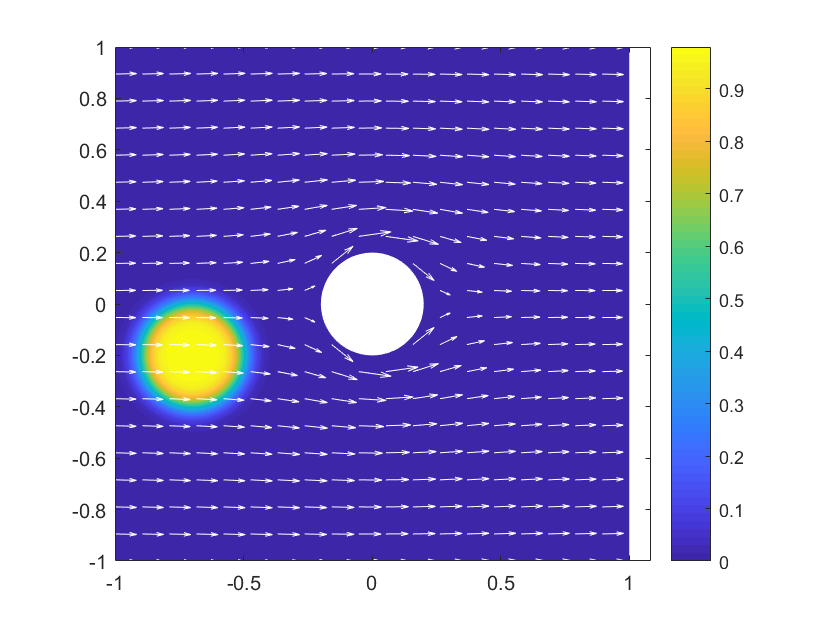
\includegraphics[width=60mm]{10}}
\subfigure[t = 5]{\label{fig:b}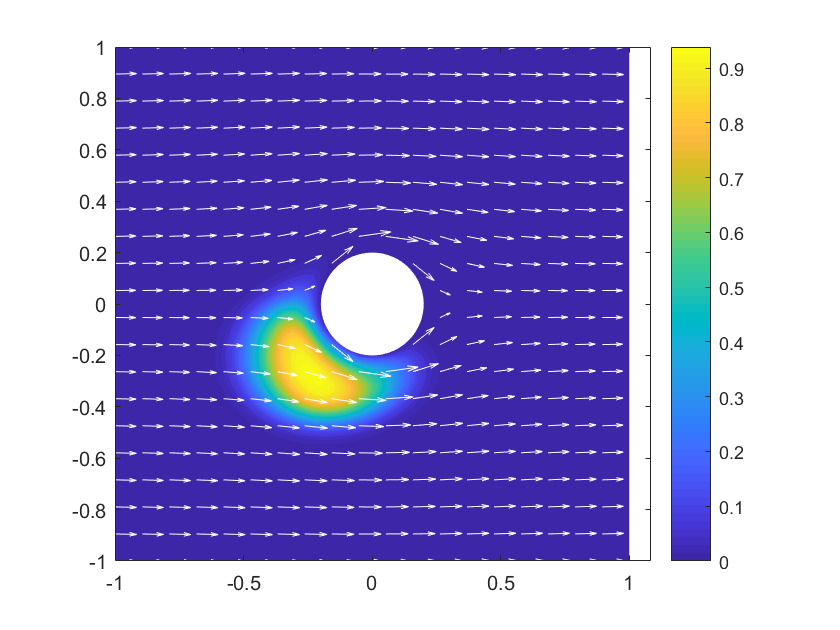
\includegraphics[width=60mm]{20}}
\subfigure[t = 10]{\label{fig:a}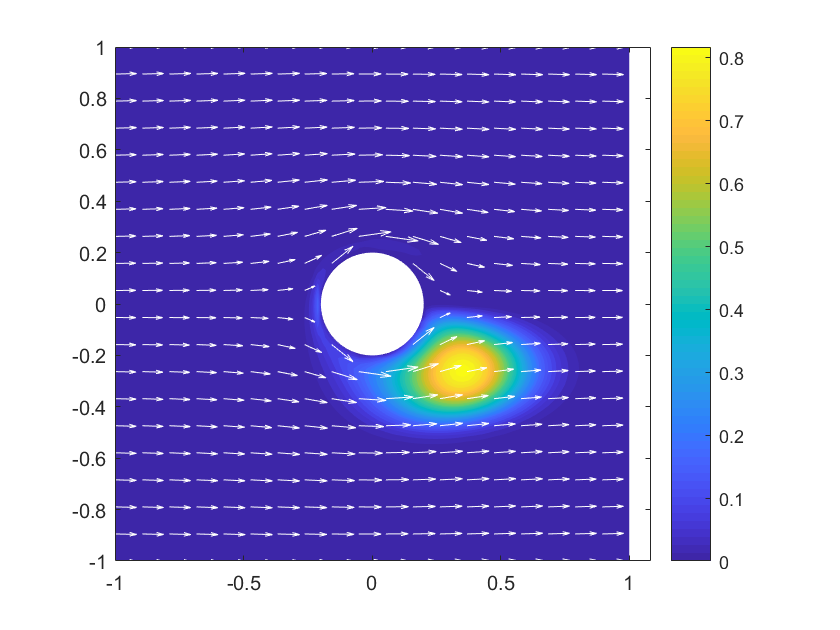
\includegraphics[width=60mm]{30}}
\subfigure[t = 15]{\label{fig:b}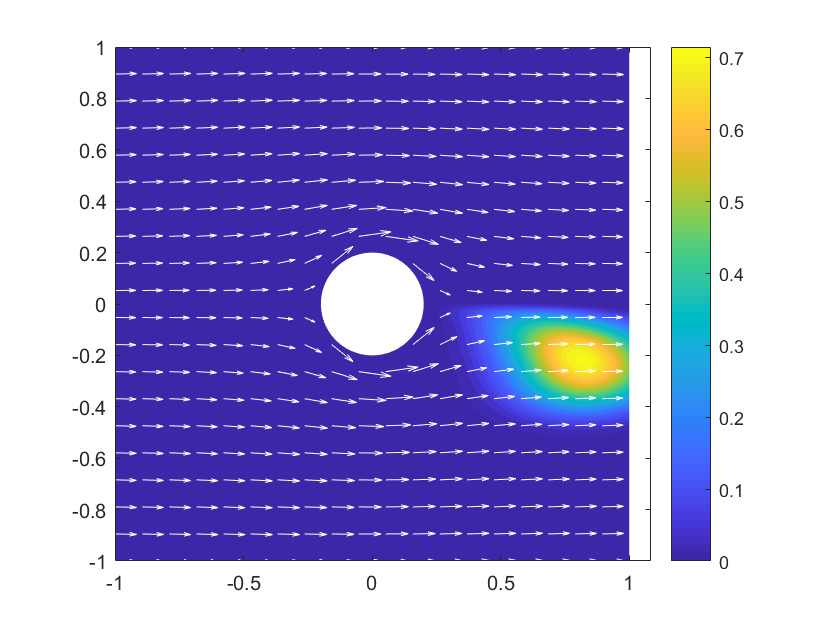
\includegraphics[width=60mm]{40}}
\caption{Flow around a rotating cylinder at $\alpha = 0$}
\end{figure}

\begin{figure}[h]
\centering    
\subfigure[t = 0]{\label{fig:a}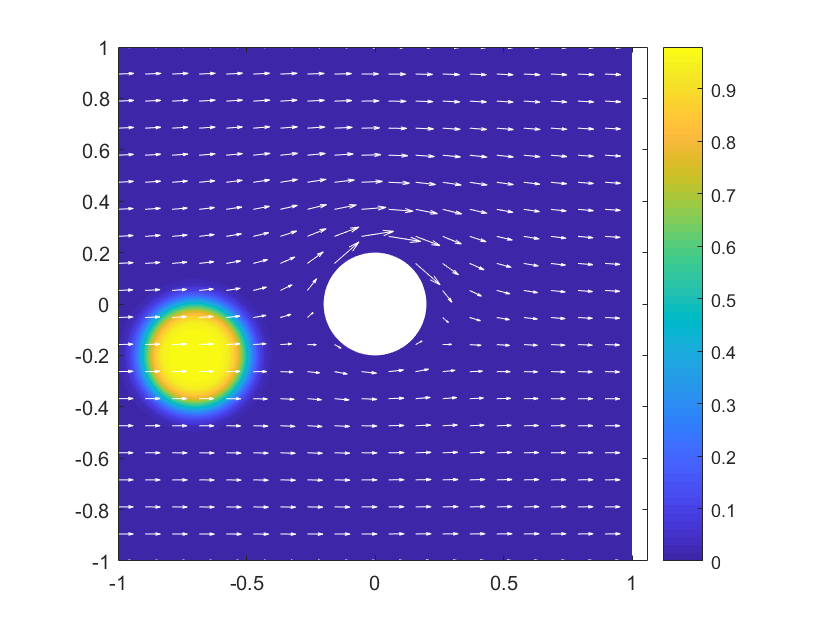
\includegraphics[width=60mm]{11}}
\subfigure[t = 5]{\label{fig:b}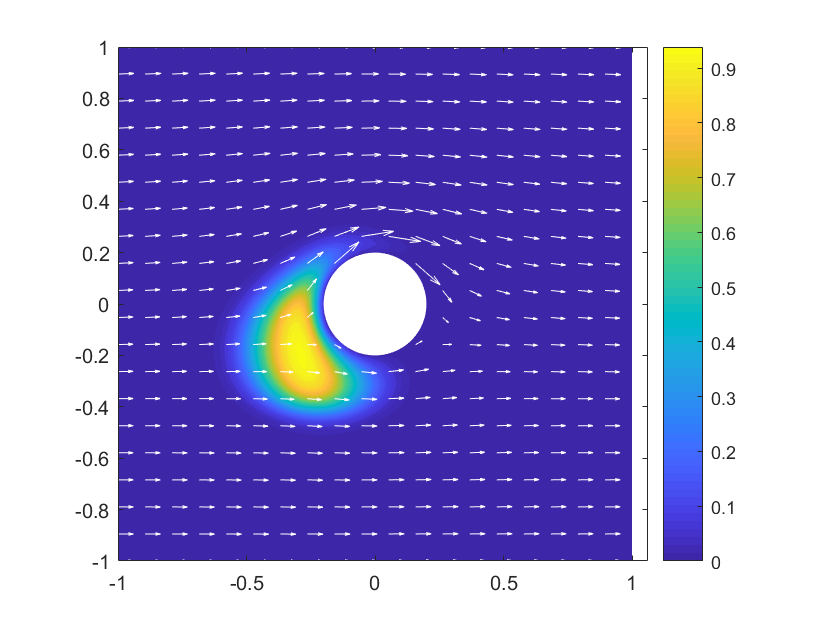
\includegraphics[width=60mm]{21}}
\subfigure[t = 10]{\label{fig:a}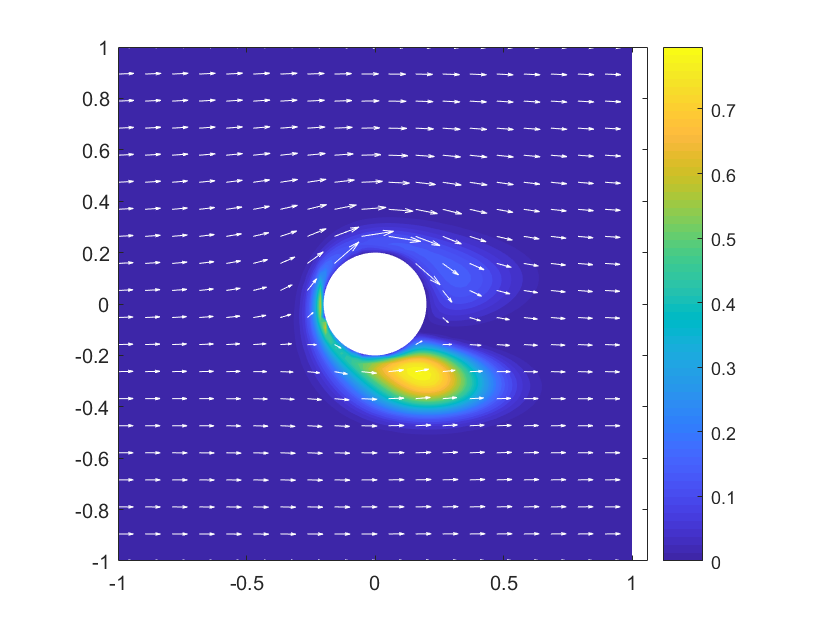
\includegraphics[width=60mm]{31}}
\subfigure[t = 15]{\label{fig:b}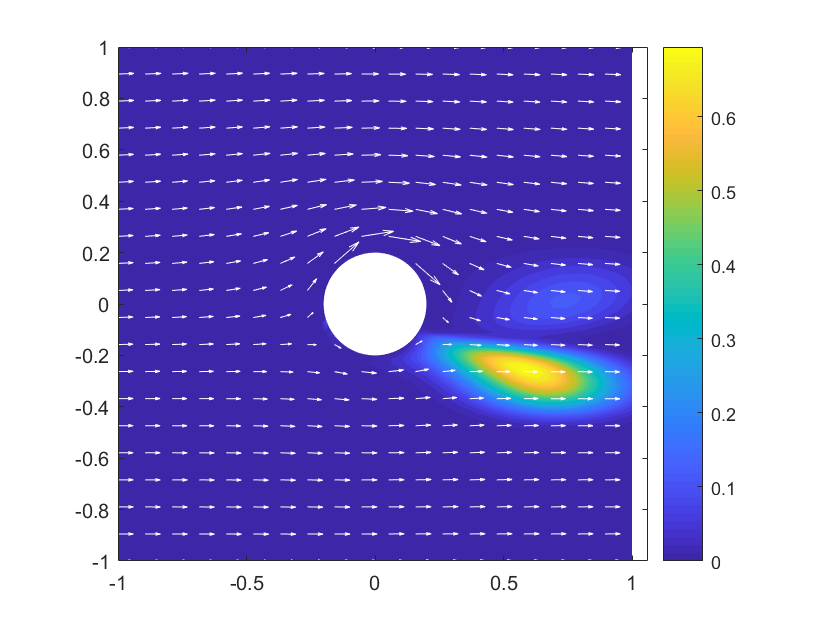
\includegraphics[width=60mm]{41}}
\caption{Flow around a rotating cylinder at $\alpha = 0.1$}
\end{figure}

\begin{figure}[h]
\centering    
\subfigure[t = 0]{\label{fig:a}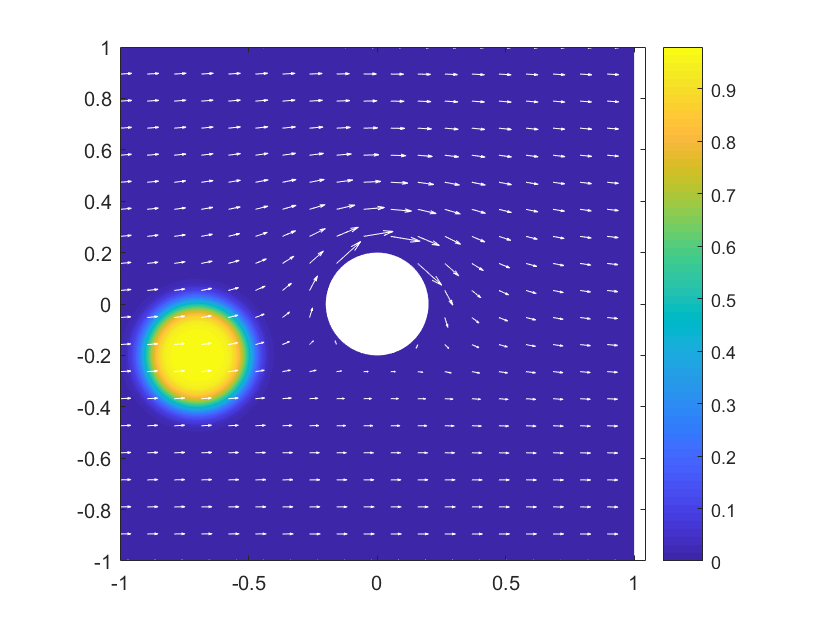
\includegraphics[width=60mm]{1}}
\subfigure[t = 5]{\label{fig:b}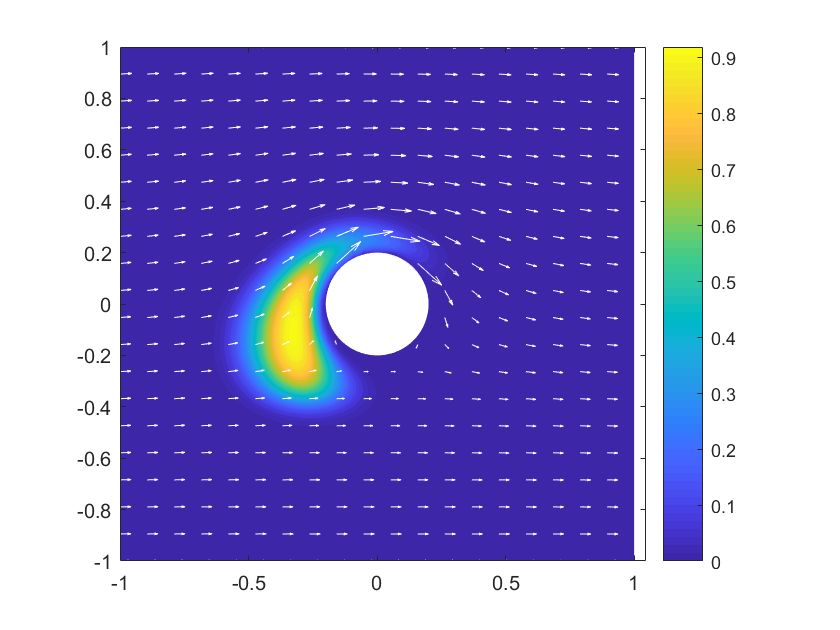
\includegraphics[width=60mm]{2}}
\subfigure[t = 10]{\label{fig:a}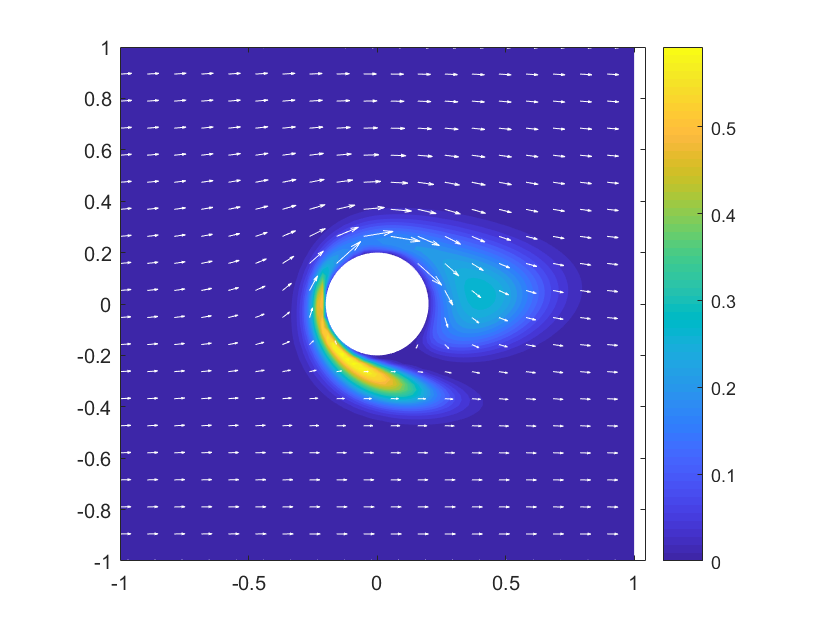
\includegraphics[width=60mm]{3}}
\subfigure[t = 15]{\label{fig:b}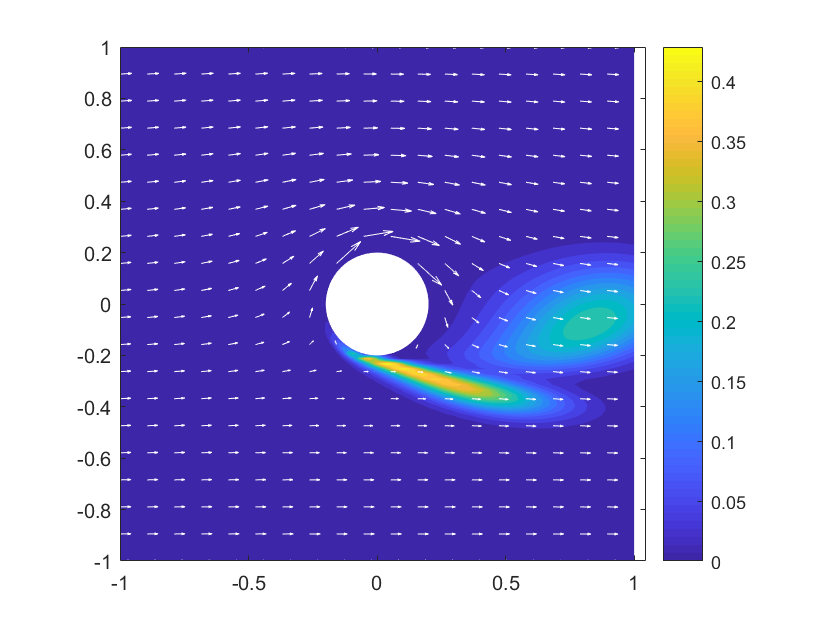
\includegraphics[width=60mm]{4}}
\caption{Flow around a rotating cylinder at $\alpha = 0.2$}
\end{figure}








%%%%%%%%%%%
\newpage
\clearpage
\setcounter{page}{1} \pagestyle{empty}
\section{References}\label{sec::References}
\begin{itemize}
\item [1] Daniil Bochkov, CS 111 - Introduction to Computational Science Homework 3 Fall 2017
\item [2] Daniil Bochkov, CS 111 - Introduction to Computational Science Lecture 10. Solving Advection Equation 2017
\item [3] Daniil Bochkov, CS 111 - Introduction to Computational Science Lecture 9. Introduction to Partial Differential Equations. 2017

\end{itemize}


%%%%%%%%%%%

\end{document}
